% Chương 3: Kiến trúc và khung quản trị niềm tin (bản rút gọn)
\chapter{KIẾN TRÚC VÀ KHUNG QUẢN TRỊ NIỀM TIN}
\label{chap:kien-truc}

Chương này trình bày phần đóng góp lý thuyết trung tâm. Nội dung đi từ yêu cầu (Mục \ref{sec:yeu-cau}) và nguyên tắc thiết kế (Mục \ref{sec:nguyen-tac}) tới kiến trúc tổng thể (Mục \ref{sec:kien-truc-tong-the}), sau đó tập trung vào khung quản trị niềm tin (Mục \ref{sec:khung-quan-tri}). Các mục tiếp theo đặc tả mô hình dữ liệu, quy trình xác minh, mô hình đe doạ và các đánh đổi.

\section{Yêu cầu hệ thống}
\label{sec:yeu-cau}

Hệ thống phải giải quyết cùng lúc hai bài toán mà Chương \ref{chap:co-so} đã chỉ ra là thuộc hai tầng khác nhau: xác minh kỹ thuật và quản trị thẩm quyền. Từ đó có năm mục tiêu thiết kế: cung cấp định danh phi tập trung cho mọi thực thể; hỗ trợ trọn vòng đời chứng thực mà không cần nơi cấp tham gia vào lúc xác minh; cho phép người học dùng một định danh với nhiều trường; bảo vệ quyền riêng tư từ gốc \cite{Cavoukian2009}; và xây dựng khung quản trị trong đó thẩm quyền được thiết lập, giới hạn, uỷ quyền lại và thu hồi theo cách bên thứ ba kiểm chứng được. Mục tiêu cuối là điểm phân biệt với một hệ thống SSI thông thường.

Các yêu cầu chức năng ở Bảng \ref{tab:v2-func} xoay quanh vòng đời chứng thực và bổ sung nhóm yêu cầu về thẩm quyền (F3--F5) mà mô hình ba bên không có. Yêu cầu phi chức năng ở Bảng \ref{tab:v2-nonfunc} được phát biểu sao cho \emph{có thể làm cho thất bại}. Chẳng hạn N4 không được đo bằng một tuyên bố về nguyên tắc, mà bằng việc liệt kê mọi trường được ghi vào hợp đồng và kiểm rằng không trường nào chứa nội dung văn bằng ở dạng đọc được.

\begin{longtable}{|c|p{3.4cm}|p{6.0cm}|p{3.0cm}|}
\caption{Yêu cầu chức năng và tiêu chí kiểm chứng}
\label{tab:v2-func} \\
\hline
\textbf{Mã} & \textbf{Yêu cầu} & \textbf{Tiêu chí kiểm chứng} & \textbf{Bằng chứng} \\ \hline
\endfirsthead
\hline
\textbf{Mã} & \textbf{Yêu cầu} & \textbf{Tiêu chí kiểm chứng} & \textbf{Bằng chứng} \\ \hline
\endhead
F1 & Đăng ký định danh & Phân giải được; băm tính lại khớp băm đã neo & Kiểm thử đầu cuối \\ \hline
F2 & Xoay khoá, giữ phiên bản & Cập nhật tăng phiên bản; chứng thực ký bằng khoá cũ vẫn kiểm được & Kiểm thử hợp đồng \\ \hline
F3 & Vòng đời thẩm quyền & Thu hồi có hiệu lực ngay ở lần xác minh kế tiếp; mọi thao tác có mã giao dịch & Kiểm thử hợp đồng, chế độ nghiêm ngặt \\ \hline
F4 & Uỷ quyền nhiều cấp & Phạm vi vượt tập cha, thời hạn vượt hạn cha đều bị từ chối; bit uỷ quyền không truyền tiếp & Kiểm thử hợp đồng \\ \hline
F5 & Chuyển quyền gốc hai bước & Quyền chỉ chuyển sau khi người được đề cử tự ký & Kiểm thử hợp đồng, mô phỏng trên chuỗi \\ \hline
F6 & Cấp phát chứng thực & Loại ngoài phạm vi bị hợp đồng từ chối & Kiểm thử hợp đồng \\ \hline
F7 & Bảo vệ khoá phía chủ thể & Không gói tin nào gửi lên dịch vụ chứa khoá riêng hay mật khẩu & Kiểm thử ví \\ \hline
F8 & Trình bày có chọn lọc & Bản trình bày chỉ chứa chứng thực được chọn, có chữ ký chủ thể & Kiểm thử đầu cuối \\ \hline
F9 & Xác minh toàn vẹn và quyền sở hữu & Phát hiện nội dung bị sửa sau khi cấp & Bộ kiểm sửa nội dung \\ \hline
F10 & Xác minh thẩm quyền độc lập & Phát hiện bên phát hành bị thu hồi hoặc hết hạn & Kiểm thử hợp đồng \\ \hline
F11 & Trạng thái chứng thực & Đơn vị hết hạn uỷ quyền vẫn thu hồi được chứng thực mình đã cấp & Kiểm thử hợp đồng \\ \hline
F12 & Dấu vết kiểm toán & Nhật ký đúng thao tác, cùng bộ tên hành động ở hai cài đặt & Kiểm thử luồng nghiệp vụ \\ \hline
\end{longtable}


\begin{longtable}{|c|p{4.4cm}|p{8.6cm}|}
\caption{Yêu cầu phi chức năng và tiêu chí đo lường}
\label{tab:v2-nonfunc} \\
\hline
\textbf{Mã} & \textbf{Yêu cầu} & \textbf{Tiêu chí đo lường} \\ \hline
\endfirsthead
\hline
\textbf{Mã} & \textbf{Yêu cầu} & \textbf{Tiêu chí đo lường} \\ \hline
\endhead
N1 & Thẩm quyền kiểm chứng độc lập & Tra cứu trạng thái thẩm quyền không cần tài khoản hay thoả thuận trước \\ \hline
N2 & Thay đổi quản trị để lại dấu vết & Mọi thao tác ghi sổ đăng ký có mã giao dịch; không thao tác nào xoá được lịch sử \\ \hline
N3 & Quy tắc thi hành ở nơi không bỏ qua được & Gọi thẳng hợp đồng, bỏ qua tầng dịch vụ, vẫn bị chặn \\ \hline
N4 & Không đọc được thông tin học thuật từ chuỗi & Không trường nào trên chuỗi chứa nội dung văn bằng ở dạng đọc được. Tiêu chí này \emph{không} đồng nghĩa với ``không có dữ liệu cá nhân trên chuỗi'' (Mục \ref{sec:tn-oracle}) \\ \hline
N5 & Khoá riêng không rời thiết bị & Không gói tin nào chứa khoá riêng, mật khẩu hay cụm từ khôi phục \\ \hline
N6 & Phát hiện kịch bản gian lận định nghĩa trước & Mỗi kịch bản ở Bảng \ref{tab:v2-threat} bị chặn, và thông điệp từ chối khớp đúng nguyên nhân \\ \hline
N7 & Xác minh không cần nơi cấp trực tuyến & Hoàn tất khi dịch vụ của bên phát hành ngừng, chỉ cần chuỗi và lớp lưu trữ \\ \hline
N8 & Tuân thủ W3C DID Core và VC & Cấu trúc hợp lệ theo đặc tả \cite{W3C_DIDCore2022, W3C_VCDM2025}; điểm chưa tuân thủ được liệt kê \\ \hline
N9 & Hợp đồng giao diện ổn định & Hai cài đặt trả cùng kết quả, cùng mã trạng thái, kể cả với đầu vào sai \\ \hline
N10 & Thời gian xác minh chấp nhận được & Phân vị 95 của tuyến đọc dưới 500\,ms khi có tải đồng thời \\ \hline
N11 & Không lỗi chức năng dưới tải & Không yêu cầu nào thất bại trong toàn bộ phép đo \\ \hline
N12 & Chi phí ví chấp nhận được & Mở khoá ví dưới 1 giây trên thiết bị phổ thông; một lần ký dưới 10\,ms \\ \hline
\end{longtable}


\section{Nguyên tắc thiết kế}
\label{sec:nguyen-tac}

\textbf{Phi tập trung có kiểm soát.} Hệ thống bỏ điểm xác minh trung tâm nhưng giữ một nguồn niềm tin gốc lo việc quản trị thẩm quyền. Quyền lực của nguồn gốc này bị giới hạn rõ: nó quyết định ai được cấp loại văn bằng nào, nhưng không giữ dữ liệu người học, không tham gia từng lần xác minh và không có khả năng kỹ thuật để ký thay bất kỳ bên phát hành nào. Thể chế giữ đúng phần quyền lực mà nó thật sự cần.

\textbf{Phân lớp với phụ thuộc một chiều.} Lớp trên phụ thuộc lớp dưới, không có chiều ngược lại. Nhờ đó đổi phương thức DID không ảnh hưởng tới cấu trúc chứng thực, và chuyển từ một gốc sang mô hình liên hợp không đụng tới ba lớp dưới.

\textbf{Mọi tuyên bố phải kiểm được tại nguồn.} Giá trị băm do máy khách khai được tính lại từ nội dung; quyền hạn được kiểm trên chuỗi chứ không dựa vào vai trò ghi trong phiên đăng nhập; mọi bản ghi tham chiếu tới giao dịch đều được xác minh với nút đầy đủ trước khi ghi. Hệ quả về cấu trúc: cơ sở dữ liệu quan hệ chỉ là \emph{chỉ mục} phục vụ truy vấn nhanh, còn nguồn sự thật là trạng thái trên chuỗi.

\section{Kiến trúc tổng thể}
\label{sec:kien-truc-tong-the}

\subsection{Các thực thể và luồng hoạt động}

Hệ thống có bốn thực thể (Hình \ref{fig:v2-system-flow}). Ba thực thể đầu là mô hình ba bên của SSI; thực thể thứ tư là điểm khác biệt.

\begin{figure}[H]
    \centering
    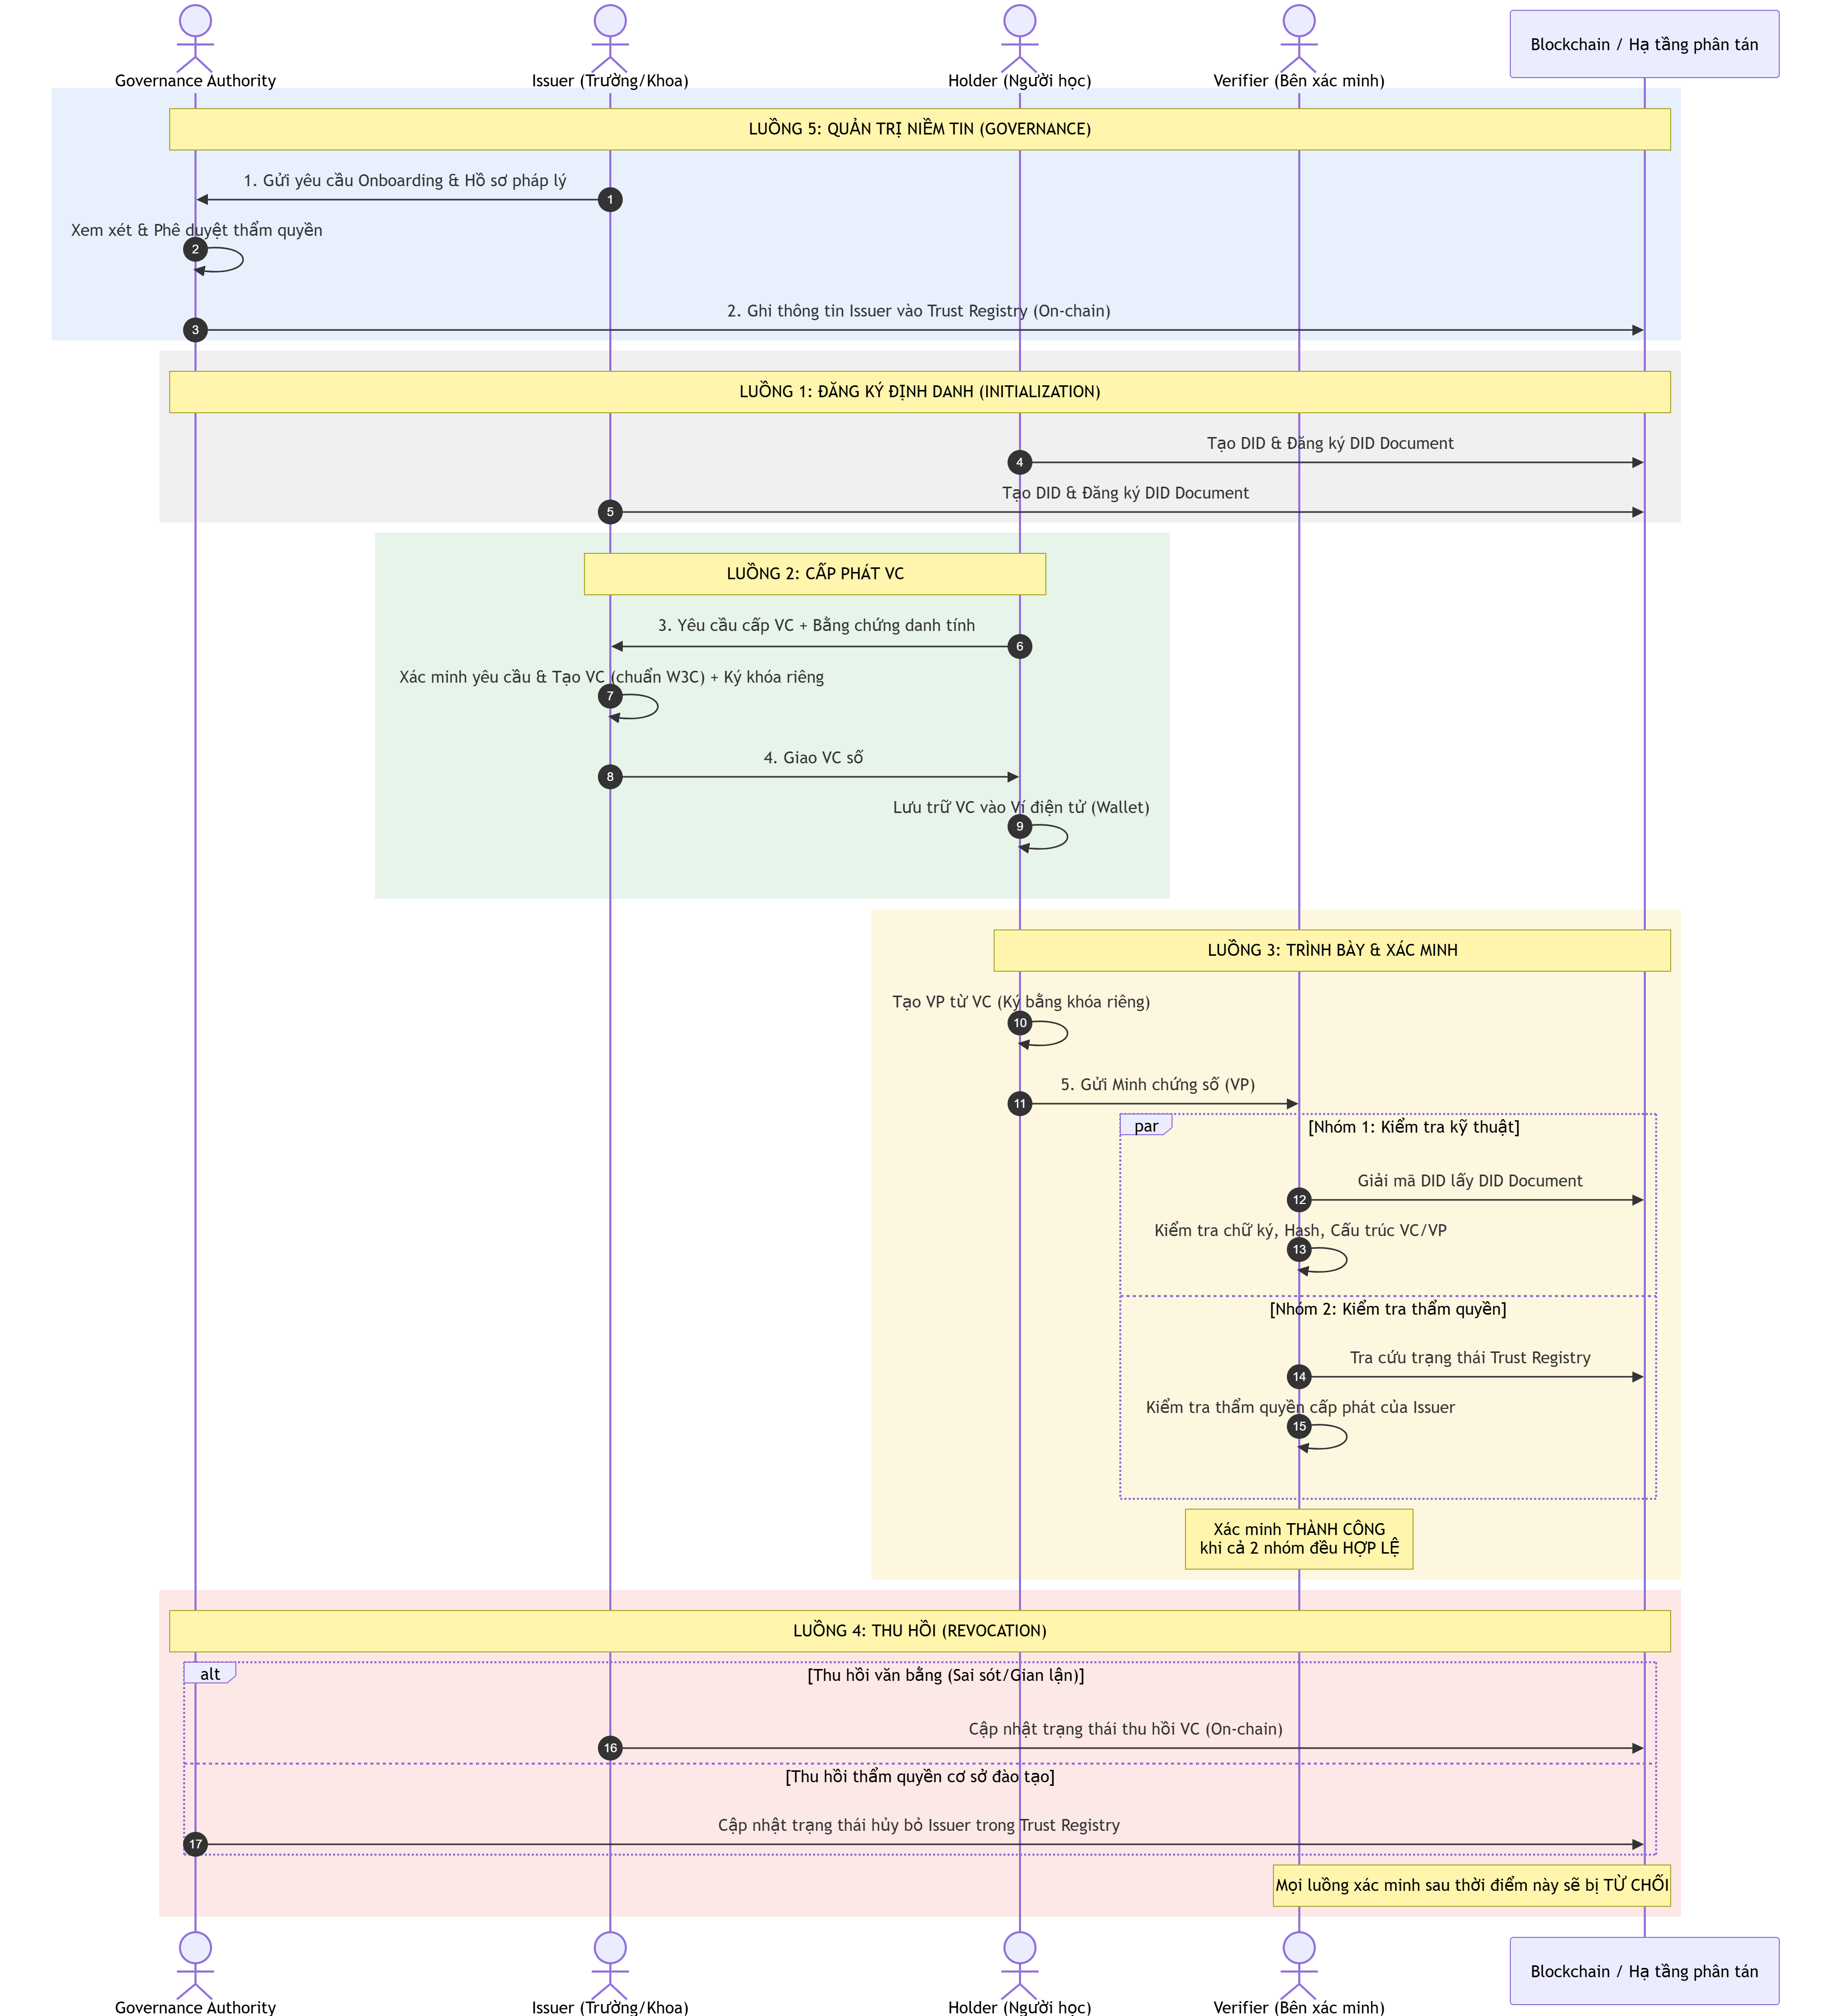
\includegraphics[width=0.66\textwidth]{images/system-flow.png}
    \caption{Luồng hoạt động giữa bốn thực thể của hệ thống}
    \label{fig:v2-system-flow}
\end{figure}

\textit{Cơ quan quản trị} là nguồn niềm tin gốc, trong bối cảnh ĐHQGHN là cấp quản lý của ĐHQGHN hoặc đơn vị được giao về đảm bảo chất lượng. Nó không tham gia vào luồng cấp phát hay xác minh thông thường, chỉ quản lý sổ đăng ký tin cậy. \textit{Bên phát hành} là các trường thành viên được phê duyệt, mỗi trường có định danh, khoá và phạm vi thẩm quyền riêng. \textit{Chủ thể} là người học, bên duy nhất quyết định chia sẻ gì, với ai, khi nào. \textit{Bên xác minh} là bất kỳ ai cần kiểm chứng văn bằng và không cần quan hệ đặc biệt nào với các bên còn lại.

Hệ thống vận hành qua năm luồng. Luồng \textit{đăng ký định danh}: thực thể sinh khoá, dựng DID Document, ghim lên IPFS lấy định danh nội dung (CID) rồi ghi định danh cùng giá trị băm lên chuỗi. Luồng \textit{cấp phát}: bên phát hành dựng chứng thực, ký, ghim nội dung và ghi bản ghi neo; hợp đồng kiểm thẩm quyền \emph{trước khi} ghi, nên đơn vị không có quyền thất bại ngay tại bước này. Luồng \textit{trình bày và xác minh}: chủ thể ký bản trình bày; bên xác minh chạy hai nhóm kiểm tra độc lập (Mục \ref{sec:xac-minh}). Luồng \textit{thu hồi}: bên có thẩm quyền cập nhật trạng thái trên chuỗi, và mọi lần xác minh sau đó từ chối chứng thực dù chữ ký vẫn đúng. Luồng \textit{quản trị thẩm quyền} diễn ra thưa nhất nhưng có tác động dài hạn lớn nhất: cơ quan quản trị phê duyệt hoặc thu hồi bên phát hành bằng chính ví của mình, và hợp đồng là nơi quyết định thao tác có được phép hay không.

\subsection{Mô hình phân lớp và các thành phần}

Kiến trúc gồm bốn lớp (Hình \ref{fig:v2-layered}). Lớp \textit{định danh} cung cấp định danh bền vững, xoay khoá và phân giải. Lớp \textit{chứng thực} hiện thực vòng đời văn bằng. Lớp \textit{tương tác} định nghĩa giao thức trình bày và xác minh. Lớp \textit{quản trị} duy trì sổ đăng ký tin cậy và cung cấp dữ liệu để trả lời câu hỏi ``bên phát hành này có thẩm quyền không''. Trust over IP coi quản trị là một chiều xuyên suốt chứ không phải một lớp \cite{ToIP_GovMetamodel2022}; cách nhìn đó chính xác hơn về khái niệm. Ở đây quản trị vẫn được vẽ thành một lớp để ranh giới trách nhiệm trong một hệ thống cụ thể được rõ ràng.

\begin{figure}[H]
    \centering
    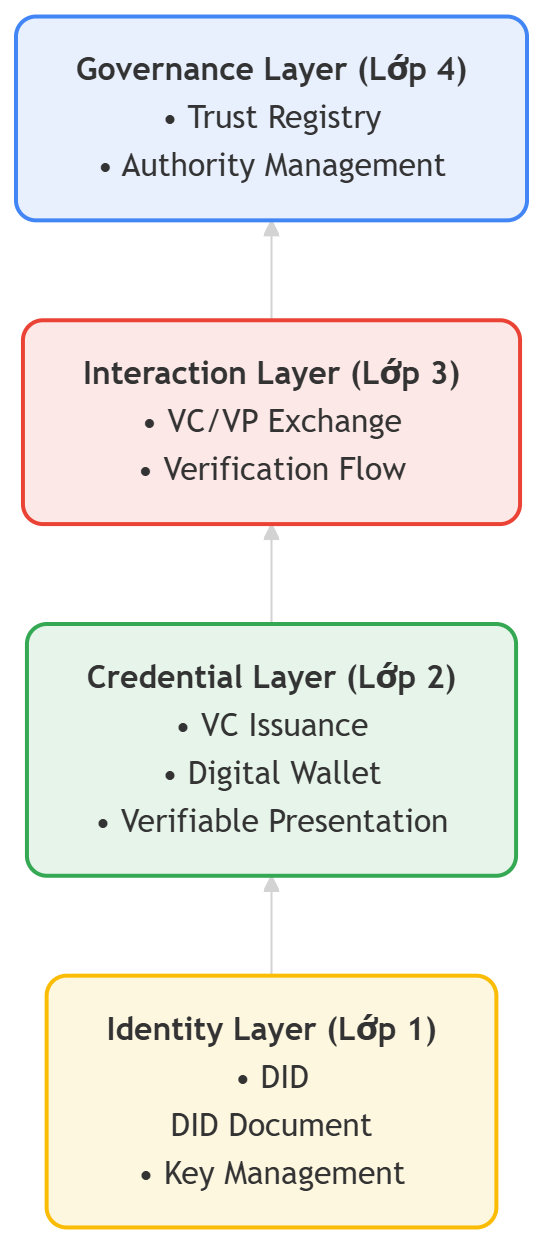
\includegraphics[width=0.26\textwidth]{images/layered_architecture.png}
    \caption{Kiến trúc phân lớp của hệ thống}
    \label{fig:v2-layered}
\end{figure}

Về quan hệ giữa các thành phần (Hình \ref{fig:v2-components}), có ba điểm cần làm rõ. Thứ nhất, ví là thành phần duy nhất chạy hoàn toàn ở máy khách: sinh khoá, mã hoá và ký đều diễn ra trong trình duyệt qua Web Cryptography API \cite{W3C_WebCrypto} và các thư viện mật mã độc lập, dữ liệu đã mã hoá lưu trong IndexedDB \cite{W3C_IndexedDB}. Tầng dịch vụ không tham gia phép mật mã nào của chủ thể. Thứ hai, tầng chỉ mục không nằm trên đường tin cậy: nếu nó trả dữ liệu sai, kết luận xác minh vẫn không bị ảnh hưởng vì mọi kết luận về tính hợp lệ đều được kiểm lại với chuỗi và với nội dung. Thứ ba, mọi thao tác ghi lên chuỗi đều do chính chủ thể ký; dịch vụ không giữ khoá của vai trò nào nên không khởi tạo được thao tác thay đổi trạng thái.

\begin{figure}[H]
    \centering
    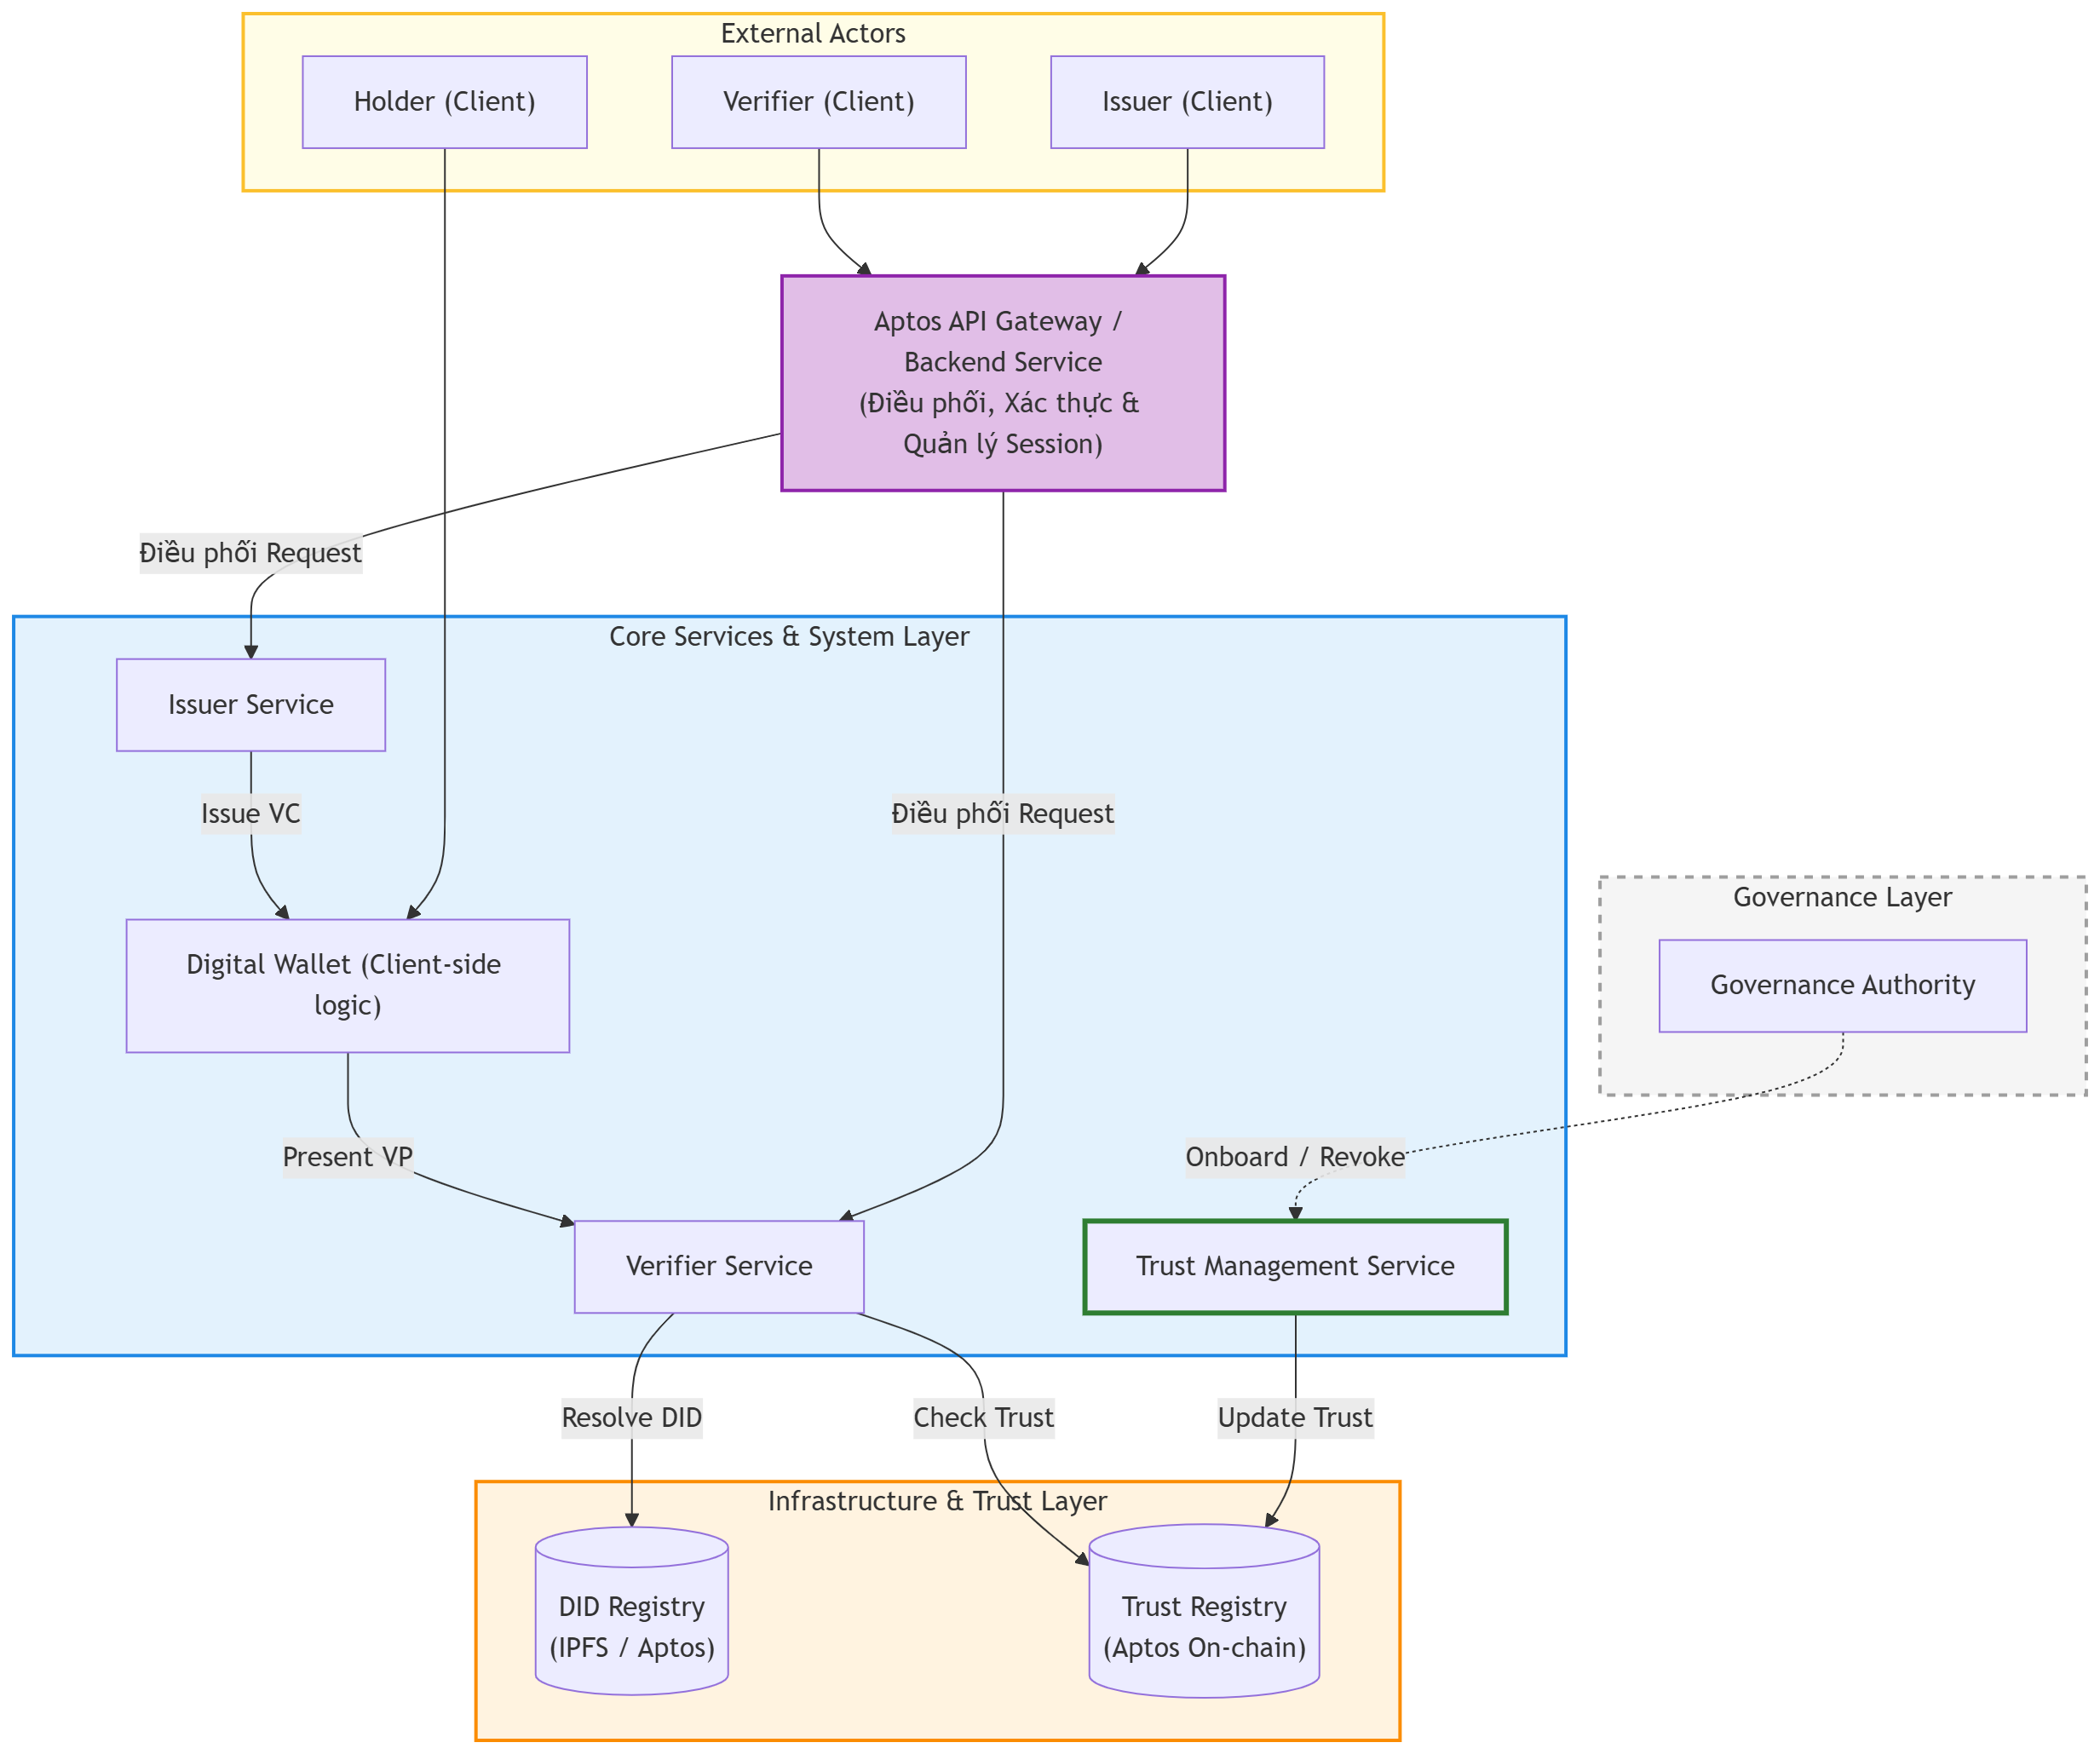
\includegraphics[width=0.92\textwidth]{images/system-architecture-components.png}
    \caption{Quan hệ giữa các thành phần của hệ thống}
    \label{fig:v2-components}
\end{figure}

\section{Khung quản trị niềm tin}
\label{sec:khung-quan-tri}

\subsection{Vấn đề khởi tạo niềm tin}

Nếu mọi niềm tin đều cần cấp trên xác nhận, cấp cao nhất lấy niềm tin từ đâu? Không từ bên trong hệ thống kỹ thuật. Mọi bằng chứng mà nguồn gốc tự tạo ra chỉ chứng minh nó giữ một khoá, điều ai cũng làm được. Thẩm quyền của ĐHQGHN đến từ sự công nhận pháp lý theo Luật Giáo dục đại học. Hệ thống kỹ thuật không thay thế sự công nhận đó mà làm cho nó \emph{kiểm chứng được}: câu hỏi thể chế ``ĐHQGHN có đáng tin không'' được chuyển thành câu hỏi kỹ thuật ``đơn vị này có đang được ĐHQGHN uỷ quyền cấp loại văn bằng này không, và tôi kiểm được điều đó mà không phải hỏi ai''. Tài liệu kỹ thuật của EBSI nêu nguyên tắc tương tự: sổ cái ghi nhận quyết định về niềm tin chứ không tạo ra chúng \cite{EBSI_TrustModel}.

\subsection{Chuỗi thẩm quyền và phạm vi cấp phát}

Thẩm quyền được biểu diễn thành chuỗi bốn mức (Hình \ref{fig:v2-chain}). \textit{Quản trị viên gốc} là duy nhất và được xác lập khi khởi tạo. Gốc cấp quyền cho các \textit{quản trị viên}; quản trị viên phê duyệt \textit{bên phát hành} kèm phạm vi; bên phát hành có bit uỷ quyền phê duyệt được \textit{bên phát hành cấp dưới} trong phạm vi hẹp hơn.

\begin{figure}[H]
    \centering
    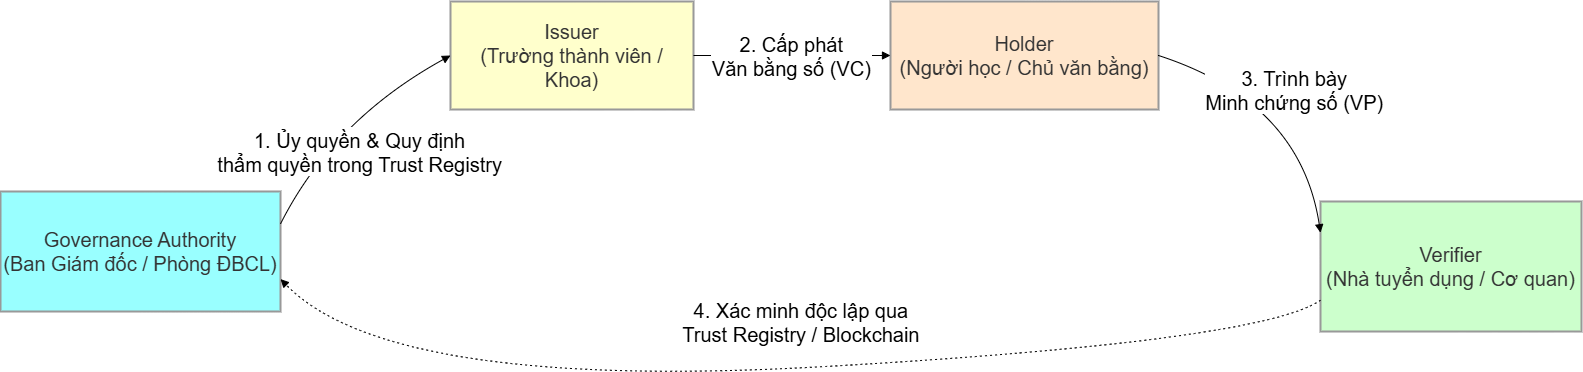
\includegraphics[width=0.9\textwidth]{images/system-interaction.png}
    \caption{Chuỗi niềm tin và các quan hệ uỷ quyền}
    \label{fig:v2-chain}
\end{figure}

Phạm vi thẩm quyền được biểu diễn bằng một mặt nạ bit (Bảng \ref{tab:v2-mask}): mỗi loại văn bằng ứng với một bit, phạm vi của một đơn vị là phép hợp các bit. Một trường được cấp bằng cử nhân, thạc sĩ và bảng điểm có $M = 1 \vee 2 \vee 8 = 11$. Câu hỏi ``đơn vị có được cấp loại $T$ không'' rút về $M \wedge T \neq 0$; câu hỏi ``phạm vi $A$ có là tập con của $B$ không'', cần cho uỷ quyền lại, rút về $A \wedge \neg B = 0$. Cả hai có chi phí hằng số, và toàn bộ phạm vi nằm gọn trong một số nguyên 64 bit. Giới hạn là số loại văn bằng tối đa bằng độ rộng số nguyên; khi vượt, cần chuyển sang nhiều từ hoặc sổ đăng ký loại theo chuỗi định danh.

\begin{table}[H]
\centering
\caption{Biểu diễn phạm vi thẩm quyền bằng mặt nạ bit}
\label{tab:v2-mask}
\renewcommand{\arraystretch}{1.2}
\small
\begin{tabular}{|c|c|p{4.8cm}|p{5.6cm}|}
\hline
\textbf{Bit} & \textbf{Giá trị} & \textbf{Loại chứng thực} & \textbf{Ghi chú} \\ \hline
0 & 1  & Bằng cử nhân, kỹ sư & \\ \hline
1 & 2  & Bằng thạc sĩ & \\ \hline
2 & 4  & Bằng tiến sĩ & \\ \hline
3 & 8  & Bảng điểm, kết quả học tập & \\ \hline
4 & 16 & Chứng nhận vi mô, chứng chỉ ngắn hạn & \\ \hline
5 & 32 & Chứng thực uỷ quyền & Chỉ quản trị viên gốc cấp được; cho phép phê duyệt bên phát hành cấp dưới \\ \hline
\end{tabular}
\end{table}


Mỗi bản ghi thẩm quyền còn mang thời hạn uỷ quyền, phản ánh đúng thực tiễn: một trường được cấp bằng trong một chu kỳ kiểm định, và thẩm quyền tự hết khi chu kỳ kết thúc nếu không được gia hạn. Giá trị không ứng với uỷ quyền vô thời hạn.

\subsection{Uỷ quyền nhiều cấp}
\label{sec:uy-quyen}

Một trường thành viên có thể cần uỷ quyền tiếp cho một khoa hay một đơn vị trực thuộc. Nếu cho uỷ quyền lại không giới hạn, chuỗi thẩm quyền mất ý nghĩa: đơn vị chỉ được cấp bằng cử nhân có thể trao cho đơn vị khác quyền cấp bằng tiến sĩ. Thiết kế đặt ba ràng buộc, cả ba do hợp đồng thi hành:

\begin{itemize}
    \item \textbf{Phạm vi phải là tập con} của phạm vi bên uỷ quyền đang có; không thể trao thứ mình không có.
    \item \textbf{Thời hạn không vượt} thời hạn của bên uỷ quyền; uỷ quyền phái sinh không sống lâu hơn uỷ quyền gốc.
    \item \textbf{Bit uỷ quyền không truyền tiếp}, nên chuỗi tối đa hai cấp. Đây là lựa chọn có chủ đích: chuỗi sâu không giới hạn khiến việc truy trách nhiệm gần như bất khả thi, trong khi lợi ích không rõ.
\end{itemize}

Một ví dụ cụ thể giúp thấy ba ràng buộc vận hành ra sao. Giả sử quản trị viên gốc phê duyệt Trường Đại học Công nghệ với phạm vi $M_A = 1 \vee 2 \vee 8 \vee 32 = 43$ (cử nhân, thạc sĩ, bảng điểm và bit uỷ quyền), thời hạn đến hết năm 2028. Trường muốn uỷ quyền cho Khoa Công nghệ thông tin cấp bảng điểm và bằng cử nhân. Bảng \ref{tab:v2-delegation} liệt kê một số yêu cầu uỷ quyền và quyết định của hợp đồng.

\begin{table}[H]
\centering
\caption{Ví dụ các yêu cầu uỷ quyền lại và quyết định của hợp đồng}
\label{tab:v2-delegation}
\renewcommand{\arraystretch}{1.2}
\small
\begin{tabular}{|p{3.4cm}|c|c|p{2.0cm}|p{4.6cm}|}
\hline
\textbf{Yêu cầu} & \textbf{Mặt nạ} & \textbf{Hạn} & \textbf{Kết quả} & \textbf{Lý do} \\ \hline
Cử nhân và bảng điểm & 9 & 2027 & Chấp nhận & $9 \wedge \neg 43 = 0$; hạn không vượt 2028 \\ \hline
Thêm bằng tiến sĩ & 13 & 2027 & Từ chối & Bit 4 không thuộc phạm vi cha: $13 \wedge \neg 43 = 4$ \\ \hline
Cử nhân, hạn 2030 & 1 & 2030 & Từ chối & Hạn vượt hạn của bên uỷ quyền \\ \hline
Cử nhân kèm bit uỷ quyền & 33 & 2027 & Từ chối & Bit uỷ quyền không truyền tiếp \\ \hline
Vô thời hạn & 1 & 0 & Từ chối & Giá trị 0 nghĩa là vô hạn, vượt hạn 2028 \\ \hline
\end{tabular}
\end{table}

Dòng cuối là một trường hợp biên dễ bị bỏ sót. Vì giá trị không mang nghĩa ``vô thời hạn'', phép so sánh thời hạn phải xử lý nó riêng; nếu chỉ so ``hạn con không lớn hơn hạn cha'' bằng số học thông thường, yêu cầu có hạn bằng không sẽ lọt qua. Hợp đồng xử lý đúng trường hợp này: khi bên uỷ quyền có thời hạn, hạn của bên được uỷ quyền phải khác không và không vượt hạn đó. Tuy vậy, bộ kiểm thử hiện chỉ có phép kiểm cho trường hợp hạn dương vượt hạn cha, chưa có phép kiểm riêng cho hạn bằng không. Đây là một ví dụ của chính nguyên tắc ở Mục \ref{sec:phuong-phap}: mã đúng nhưng chưa có phép kiểm làm nó thất bại thì chưa thể coi là đã được kiểm chứng.

Một giới hạn khác cần nêu: thu hồi thẩm quyền ở cấp trên \emph{không} tự động lan xuống cấp dưới. Hàm kiểm ``bên phát hành còn hiệu lực'' chỉ đọc bản ghi của chính bên đó, không lần ngược lên bên đã phê duyệt nó. Khi một trường bị thu hồi thẩm quyền, các khoa mà trường đã uỷ quyền vẫn cấp được văn bằng cho tới khi hết hạn hoặc bị thu hồi riêng. Ràng buộc ``hạn con không vượt hạn cha'' giới hạn thiệt hại về thời gian, nhưng không thay được cơ chế lan truyền. Bổ sung cơ chế này, bằng cách kiểm cả chuỗi phê duyệt ở bước 7 hoặc ngay trong hàm kiểm thẩm quyền, là một hướng phát triển cụ thể.

Mỗi quan hệ uỷ quyền gắn với một \emph{chứng thực uỷ quyền} do bên uỷ quyền ký; giá trị băm và CID của nó nằm trong bản ghi thẩm quyền, để bên xác minh kiểm được bằng chứng chứ không chỉ đọc một cờ trạng thái. Hợp đồng chỉ bắt buộc có chứng thực này khi thực sự có quan hệ uỷ quyền.

\subsection{Chuyển quyền gốc hai bước}

Gốc là điểm tập trung quyền lực duy nhất, nên cơ chế chuyển quyền gốc có hệ quả đặc biệt lớn. Thiết kế trực quan nhất là một thao tác trong đó gốc hiện tại chỉ định địa chỉ người kế nhiệm. Thiết kế này có một khuyết điểm chỉ lộ ra khi đã muộn: không có gì kiểm tra địa chỉ đích thật sự có người giữ khoá. Gõ nhầm một ký tự, quyền gốc rơi vào một địa chỉ không ai điều khiển. Hệ thống không sập ngay, cấp phát và xác minh vẫn chạy, nhưng năng lực quản trị mất vĩnh viễn: không phê duyệt được bên phát hành mới, không thu hồi được bên phát hành cũ, và không sửa được chính sai sót đó. Cách duy nhất là triển khai lại toàn bộ ở địa chỉ mới.

Thiết kế vì vậy tách thành \emph{đề cử} (gốc ghi địa chỉ người được đề cử vào trạng thái chờ, quyền chưa chuyển) và \emph{ký nhận} (người được đề cử tự ký để tiếp nhận), kèm thao tác \emph{huỷ đề cử}. Giá trị nằm ở chữ ký trong bước thứ hai: đó là bằng chứng mật mã duy nhất cho thấy người nhận thật sự giữ khoá của địa chỉ đã nêu. Từ đây rút ra một nguyên tắc tổng quát hơn bài toán văn bằng: \emph{khi một thao tác không thể hoàn tác, điều kiện tiên quyết của nó phải được chứng minh bằng hành động của bên bị ảnh hưởng, không phải bằng khai báo của bên thực hiện}.

\subsection{Bất đối xứng giữa cấp và thu hồi}
\label{sec:bat-doi-xung}

Cách thiết kế tự nhiên là đối xứng: cần thẩm quyền còn hiệu lực để cấp thì cũng cần thẩm quyền còn hiệu lực để thu hồi. Xét kịch bản sau. Một trường có thẩm quyền tới hết năm 2026. Năm 2027 trường phát hiện một văn bằng cấp năm 2025 là kết quả gian lận. Với thiết kế đối xứng, trường không thu hồi được vì thẩm quyền đã hết hạn, và văn bằng gian lận tiếp tục qua mọi phép xác minh. Tình huống tương tự xảy ra khi thẩm quyền của một trường bị thu hồi vì sai phạm: đúng lúc cần thu hồi văn bằng nhất thì năng lực thu hồi bị khoá.

Nguyên tắc rút ra là \emph{thao tác thu hồi luôn phải dễ hơn thao tác cấp}. Cấp phát đòi hỏi thẩm quyền còn hiệu lực và loại nằm trong phạm vi. Thu hồi chỉ đòi hỏi quyền sở hữu (đúng bên đã cấp) và định danh còn hoạt động. Chứng thực đã hết hạn vẫn thu hồi được, vì hết hạn nói rằng chứng thực không còn giá trị \emph{từ một thời điểm}, còn thu hồi nói rằng nó \emph{chưa bao giờ} đáng tin. Phát biểu tổng quát: trong hệ thống an toàn, thao tác làm giảm quyền nên có điều kiện lỏng hơn thao tác làm tăng quyền; điều kiện chặt ở thao tác giảm không bảo vệ hệ thống mà chỉ ngăn hệ thống tự sửa sai.

\subsection{Dấu vết kiểm toán và phân tách thẩm quyền}

Hai yêu cầu có vẻ đối lập cần được xử lý cùng nhau: mọi thay đổi quản trị phải để lại dấu vết không xoá được, và một đơn vị bị thu hồi phải có thể được cấp lại sau khi khắc phục. Ghi đè bản ghi cũ thì mất dấu vết; cấm cấp lại thì không phản ánh được thực tiễn. Thiết kế tách hai thứ: bảng tra ``đơn vị $A$ hiện ứng với bản ghi nào'' được cập nhật, còn bản ghi cũ vẫn nằm nguyên, và mỗi bản ghi mang số \emph{phiên bản} tăng dần. Lịch sử đầy đủ của một đơn vị vì thế luôn truy được, trong khi tra trạng thái hiện tại vẫn là một phép tra trực tiếp. Định danh cũng theo cơ chế này: khi lộ khoá, chủ thể thu hồi định danh cũ và đăng ký định danh mới; định danh cũ vẫn tra ra trạng thái ``đã thu hồi'' để các chứng thực ký bằng khoá cũ phản ánh đúng.

Bảng \ref{tab:v2-role} quy định thao tác nào thuộc vai trò nào. Có hai quy định cần giải thích. Kích hoạt lại một chứng thực bị đình chỉ chỉ thuộc quản trị viên, dù chính bên phát hành đã đình chỉ nó; nếu không, việc đình chỉ có thể được hoàn tác bất cứ lúc nào mà không ai biết. Ký nhận quyền gốc không bị chặn theo vai trò, vì tại thời điểm ký người được đề cử chưa phải là gốc; rào chắn thật là điều kiện trùng địa chỉ trong hợp đồng.

\begin{table}[H]
\centering
\caption{Phân tách thẩm quyền theo thao tác}
\label{tab:v2-role}
\renewcommand{\arraystretch}{1.2}
\small
\begin{tabular}{|p{4.4cm}|p{3.4cm}|p{5.6cm}|}
\hline
\textbf{Thao tác} & \textbf{Vai trò được phép} & \textbf{Cơ sở} \\ \hline
Cấp, thu hồi quyền quản trị viên; cấp bit uỷ quyền & Chỉ quản trị viên gốc & Hai quyền có hệ quả rộng nhất phải tập trung ở gốc \\ \hline
Phê duyệt bên phát hành & Gốc, quản trị viên & Thao tác thường xuyên, cần phân cấp \\ \hline
Phê duyệt bên phát hành cấp dưới & Bên phát hành có bit uỷ quyền & Ba ràng buộc ở Mục \ref{sec:uy-quyen} \\ \hline
Đề cử, huỷ đề cử quyền gốc & Chỉ quản trị viên gốc & Gốc hiện tại quyết định người kế nhiệm \\ \hline
Ký nhận quyền gốc & Địa chỉ đang được đề cử & Không chặn theo vai trò; rào chắn là điều kiện trùng địa chỉ trong hợp đồng \\ \hline
Cấp phát chứng thực & Bên phát hành còn hiệu lực, loại trong phạm vi & Điều kiện chặt nhất hệ thống \\ \hline
Thu hồi, đình chỉ chứng thực & Bên đã cấp chứng thực đó & Chỉ cần quyền sở hữu (Mục \ref{sec:bat-doi-xung}) \\ \hline
Kích hoạt lại chứng thực & Gốc, quản trị viên & Bên phát hành tự ngưng rồi tự bật thì việc ngưng mất giá trị kiểm toán \\ \hline
Tự đình chỉ, tự mở định danh & Chủ định danh & Ghi lại ai đã đặt trạng thái để phân biệt với bị quản trị viên khoá \\ \hline
\end{tabular}
\end{table}


\section{Mô hình dữ liệu trên chuỗi và ngoài chuỗi}
\label{sec:mo-hinh-du-lieu}

\subsection{Nguyên tắc phân chia và mức bảo vệ đạt được}

Lên chuỗi là những dữ liệu cần bất biến và đọc tự do: định danh cùng CID và giá trị băm của DID Document; bản ghi thẩm quyền gồm phạm vi, thời hạn, trạng thái; giá trị băm định danh chứng thực, CID, giá trị băm nội dung và trạng thái. Mọi trường đều là giá trị băm, định danh kỹ thuật, cờ trạng thái hoặc dấu thời gian. Ngoài chuỗi là nội dung đầy đủ của DID Document và chứng thực. Hệ thống lưu \emph{giá trị băm} của định danh chứng thực chứ không lưu bản thân định danh, đủ để tra cứu mà không lộ định danh cho người quan sát ngẫu nhiên.

Từng có lập luận rằng vì mọi trường đều là giá trị băm nên trên chuỗi không có dữ liệu cá nhân. Như Mục \ref{sec:blockchain} đã phân tích, lập luận này không đứng vững \cite{EDPB2025}. Địa chỉ tài khoản của chủ thể là một định danh giả danh liên kết được với con người cụ thể nếu có thêm thông tin phụ, và giá trị băm nội dung không muối là một máy xác nhận. Mục \ref{sec:tn-oracle} đo mức nguy hiểm của máy xác nhận này và cho một kết quả hai mặt. Định danh chứng thực là một UUID ngẫu nhiên 122 bit nằm trong nội dung được băm, nên với kẻ chỉ có dữ liệu trên chuỗi, nó đóng vai trò như một muối ngẫu nhiên. Nhưng ai đã biết định danh ấy thì khôi phục được các thuộc tính có không gian giá trị nhỏ gần như tức thì. Phát biểu đúng mức vì vậy là: kiến trúc \emph{giảm đáng kể} mức phơi nhiễm so với ghi nội dung lên chuỗi, nhưng \emph{không} bảo đảm quyền xoá.

Bản thử nghiệm ghim nội dung chứng thực lên IPFS ở dạng không mã hoá. Mô hình an toàn thực tế vì thế dựa vào việc CID không được công bố, tức là bảo mật nhờ khó đoán chứ không phải bảo mật bằng mật mã. Thiết kế đầy đủ cần mã hoá nội dung bằng khoá công khai của chủ thể trước khi ghim.

\subsection{Phương thức định danh \texttt{did:vnu}}

Cú pháp tuân theo DID Core \cite{W3C_DIDCore2022}:

\begin{lstlisting}
    did:vnu:<loai-thuc-the>:<dia-chi-tai-khoan>
    vi du:  did:vnu:issuer:0x1a2b...ef12
\end{lstlisting}

 Vì phần định danh là địa chỉ tài khoản, chủ thể kiểm soát định danh bằng chính cặp khoá dùng để ký giao dịch. Thành phần loại thực thể chỉ là nhãn mô tả lúc đăng ký: khi một người học được phê duyệt làm bên phát hành, định danh cũ không phản ánh vai trò mới, nên nhãn này không bao giờ được dùng làm căn cứ phân quyền; thẩm quyền luôn được tra từ sổ đăng ký theo địa chỉ.

Phân giải gồm bốn bước (Hình \ref{fig:v2-did-resolution}): tách địa chỉ; truy vấn hợp đồng lấy CID, giá trị băm, phiên bản và trạng thái; tải tài liệu từ IPFS; tính lại giá trị băm và đối chiếu với giá trị đã neo. Bước cuối loại bỏ sự phụ thuộc vào cổng IPFS trung gian: dù cổng nào trả dữ liệu, sự không nhất quán vẫn bị phát hiện. Khi xoay khoá, chủ thể ghim DID Document mới rồi gọi thao tác cập nhật bằng chữ ký của khoá \emph{hiện tại}; hợp đồng tăng số phiên bản và giữ các phiên bản cũ. Thao tác cập nhật nhận thêm phiên bản kỳ vọng để phát hiện hai cập nhật đồng thời ghi đè lên nhau.

\begin{figure}[H]
    \centering
    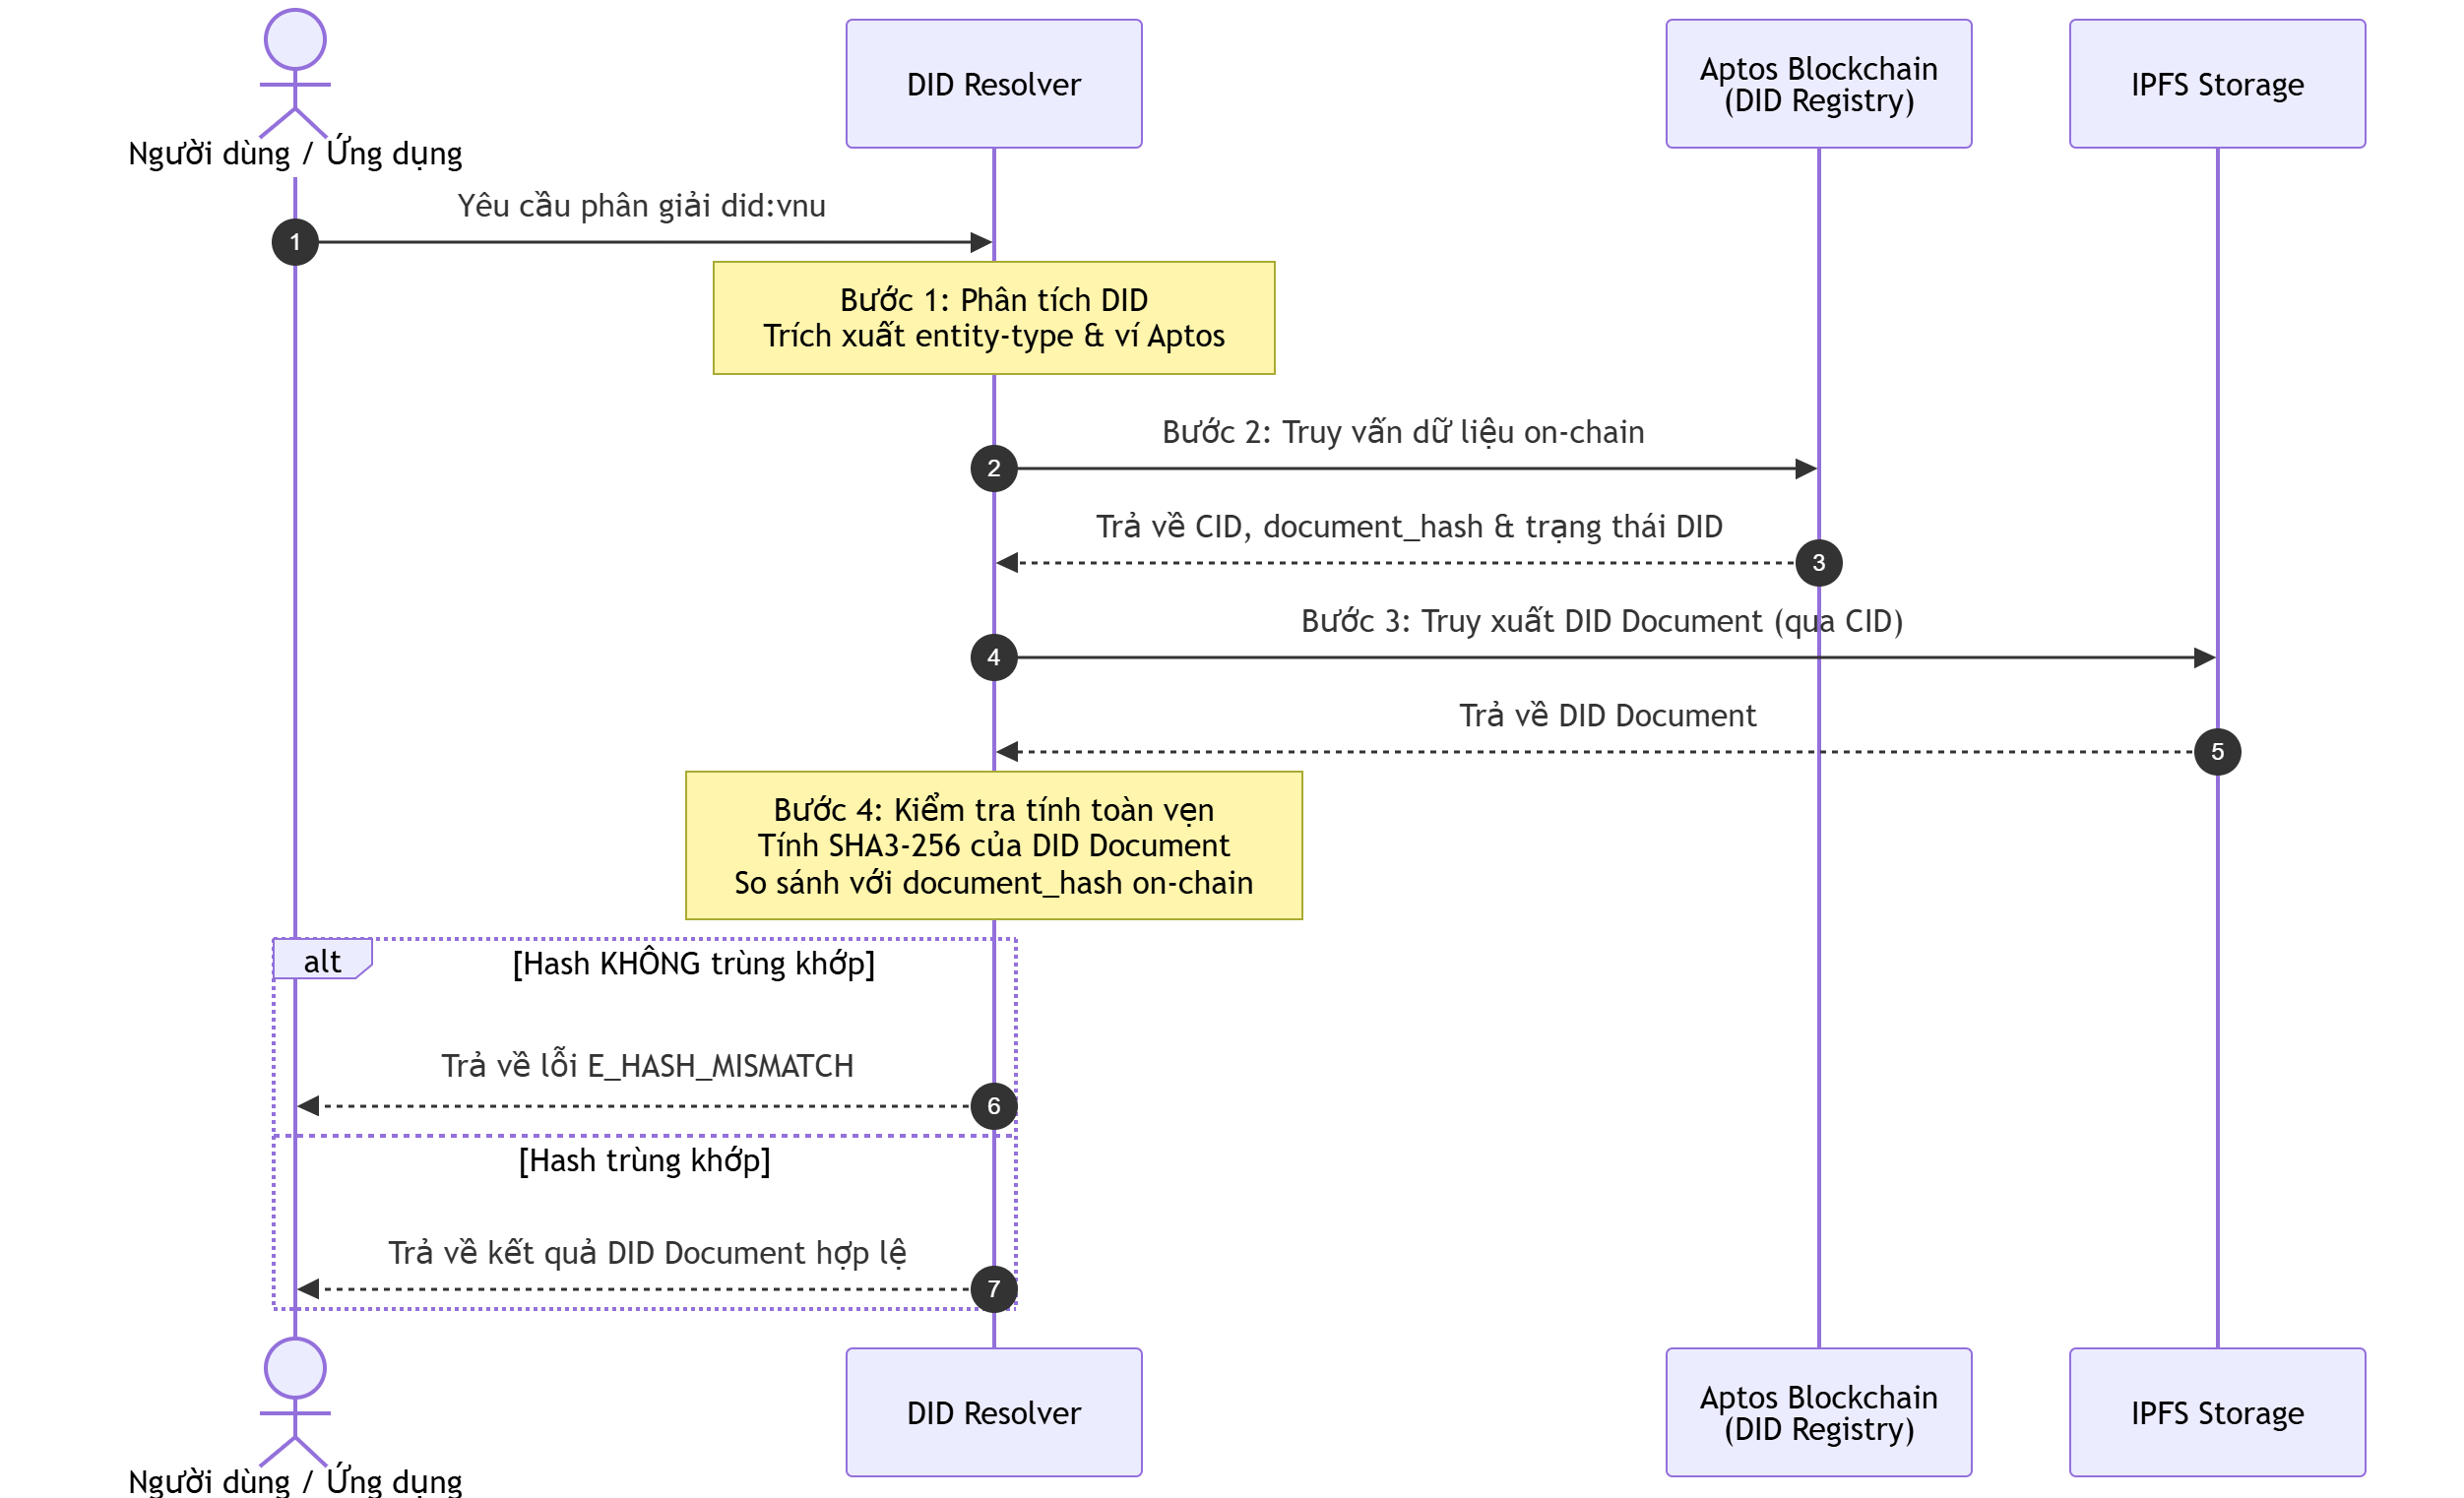
\includegraphics[width=0.82\textwidth]{images/did-resolution.png}
    \caption{Quy trình phân giải định danh \texttt{did:vnu}}
    \label{fig:v2-did-resolution}
\end{figure}

\section{Quy trình xác minh bảy bước}
\label{sec:xac-minh}

Mỗi bước kiểm một tính chất độc lập và báo kết quả riêng, để bên xác minh biết chính xác vì sao một chứng thực bị từ chối. Bảy bước chia thành hai nhóm (Hình \ref{fig:v2-seq-verify}).

\begin{figure}[H]
    \centering
    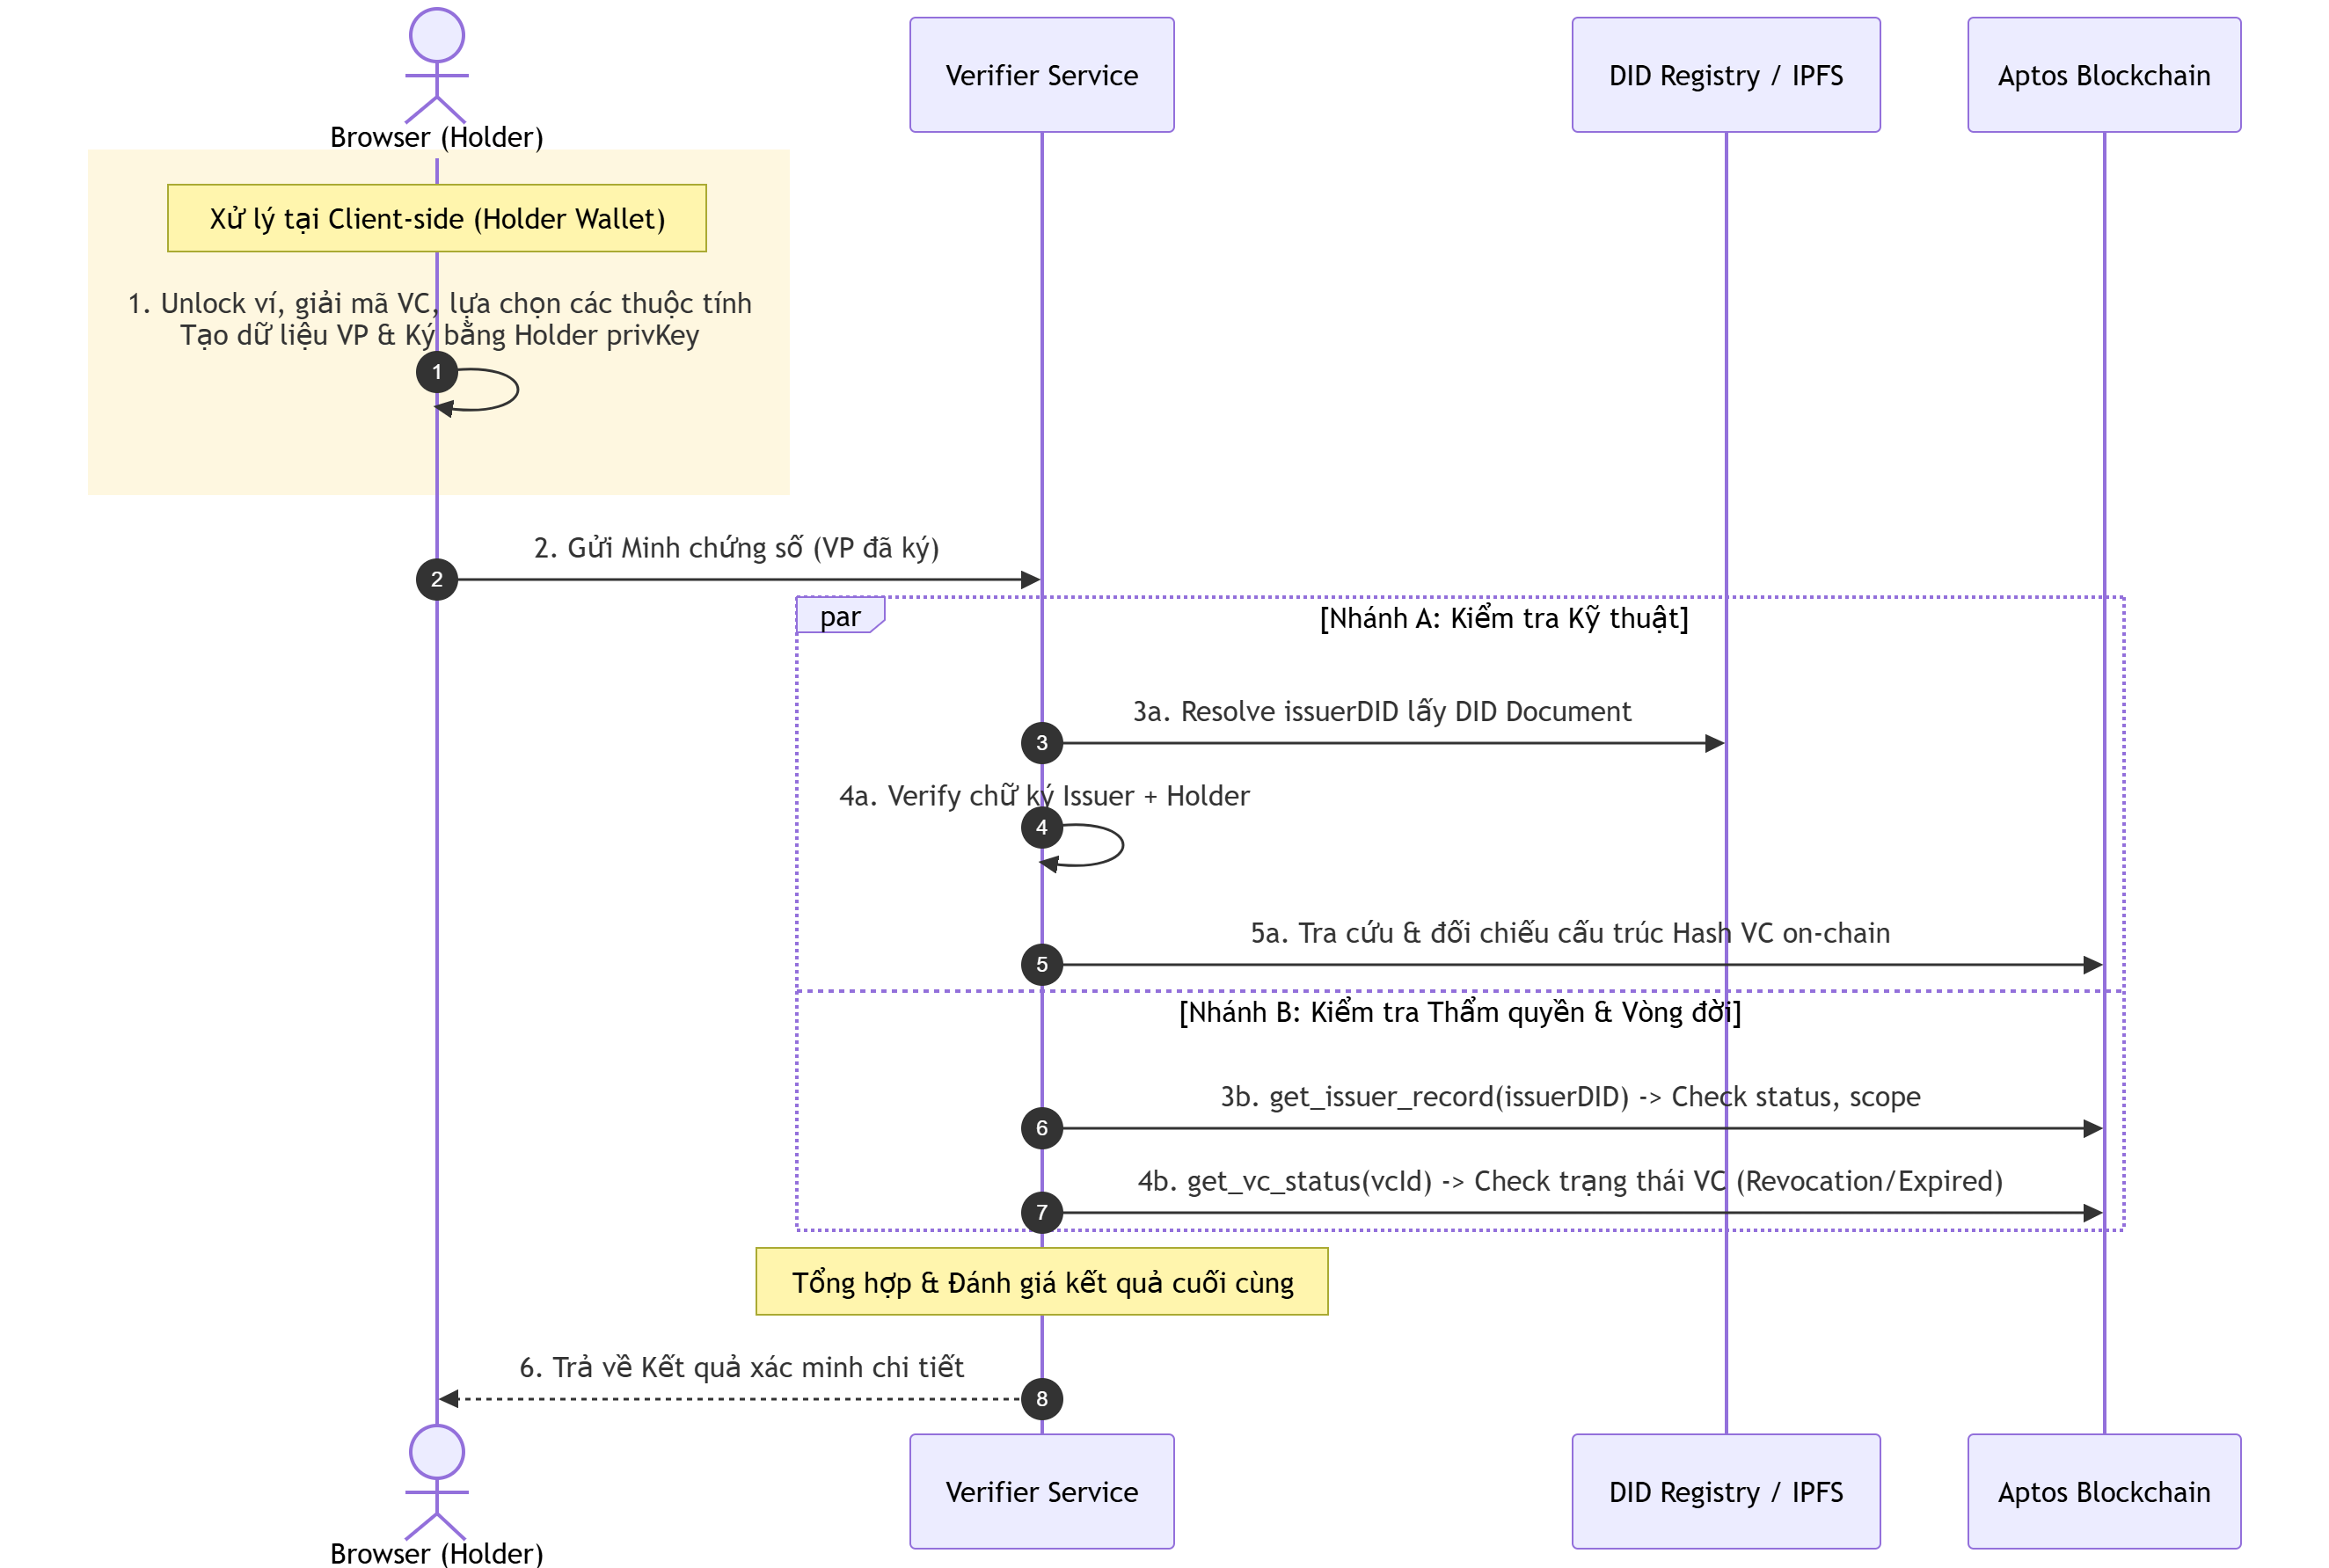
\includegraphics[width=0.95\textwidth]{images/seq_xac_minh_vp.png}
    \caption{Sơ đồ tuần tự trình bày và xác minh}
    \label{fig:v2-seq-verify}
\end{figure}

\textit{Nhóm kỹ thuật.} (1) Tải bản trình bày từ IPFS theo CID; thất bại ở đây nghĩa là dữ liệu không khả dụng, khác với dữ liệu không hợp lệ. (2) Tính lại giá trị băm của bản trình bày và đối chiếu. (3) Kiểm chữ ký trên bản trình bày bằng khoá công khai của chủ thể, để xác lập người trình bày đúng là chủ thể. (4) Phân giải định danh của chủ thể và kiểm nó còn hoạt động.

\textit{Nhóm thẩm quyền và trạng thái.} (5) Kiểm trạng thái hiệu lực của từng chứng thực, kể cả thời điểm hết hạn. (6) Tính lại giá trị băm nội dung của từng chứng thực và đối chiếu với giá trị đã neo trên chuỗi lúc cấp. (7) Tra trạng thái thẩm quyền của bên phát hành từng chứng thực.

Bước 6 là bước mà hệ thống chỉ theo dõi trạng thái không có. Bước 5 trả lời ``chứng thực còn hiệu lực không'', nhưng không phát hiện được việc nội dung bị sửa sau khi cấp: sửa điểm trung bình rồi ghim lại thì trạng thái trên chuỗi vẫn là ``đang hiệu lực'', và cả bước 5 lẫn bước 7 đều đạt. Chỉ có phép đối chiếu với giá trị băm đã neo phát hiện được. Mục \ref{sec:dg-chuc-nang} trình bày bộ kiểm thử dựng đúng kịch bản này.

Kết quả là hợp lệ khi và chỉ khi cả bảy bước đạt, nhưng báo cáo trả trạng thái từng bước, vì ba loại thất bại ở Bảng \ref{tab:v2-verif-matrix} cần ba cách xử lý khác nhau: nội dung bị sửa là gian lận chủ động; chứng thực bị thu hồi là tình huống hành chính bình thường; bên phát hành mất thẩm quyền thì nội dung có thể vẫn đúng nhưng giá trị thể chế cần xem lại.

\begin{table}[H]
\centering
\caption{Ma trận kết quả xác minh}
\label{tab:v2-verif-matrix}
\renewcommand{\arraystretch}{1.2}
\small
\begin{tabular}{|p{2.2cm}|p{2.4cm}|p{1.6cm}|p{7.0cm}|}
\hline
\textbf{Nhóm kỹ thuật} & \textbf{Nhóm thẩm quyền} & \textbf{Kết quả} & \textbf{Ý nghĩa với bên xác minh} \\ \hline
Đạt & Đạt & Hợp lệ & Hợp lệ cả về nội dung lẫn thẩm quyền \\ \hline
Không đạt & Đạt & Từ chối & Nội dung bị sửa, chữ ký sai hoặc người khác trình bày: dấu hiệu gian lận chủ động \\ \hline
Đạt & Không đạt (bước 5) & Từ chối & Nội dung nguyên vẹn nhưng chứng thực đã bị thu hồi, đình chỉ hoặc hết hạn; báo cáo chỉ rõ nguyên nhân \\ \hline
Đạt & Chỉ bước 7 không đạt & Hợp lệ, kèm cảnh báo & Nơi cấp đã mất thẩm quyền sau khi cấp; văn bằng vẫn là văn bằng thật, đang chờ cấp trên xem xét \\ \hline
Không đạt & Không đạt & Từ chối & Liệt kê đủ các bước hỏng, không dừng ở bước đầu \\ \hline
\end{tabular}
\end{table}


\section{Mô hình đe doạ}
\label{sec:de-doa}

Mô hình giả định kẻ tấn công gửi được yêu cầu bất kỳ tới tầng dịch vụ, đọc được mọi dữ liệu công khai trên chuỗi và trên IPFS khi biết CID, và kiểm soát một tài khoản hợp lệ của chính mình. Mô hình \emph{không} giả định kẻ tấn công chiếm được khoá của người khác, chạy được mã trong trình duyệt của người khác, hay làm sai lệch trạng thái chuỗi. Riêng trường hợp khoá của một bên phát hành bị lộ cần nêu rõ: mỗi bên phát hành ký bằng một khoá duy nhất, nên kẻ chiếm được khoá cấp được chứng thực hợp lệ trong toàn bộ phạm vi của đơn vị cho tới khi thẩm quyền bị thu hồi. Đây là đặc điểm chung của các hệ thống chữ ký đơn \cite{Saramago2021}. Thiết kế chỉ giảm nhẹ một phần: thẩm quyền có thời hạn và phạm vi nên thiệt hại bị chặn trên, và mọi chứng thực đã cấp đều thu hồi được.

Mô hình do chính nghiên cứu định nghĩa, nên chặn hết các hành vi trong đó là \emph{điều kiện cần}, chưa phải điều kiện đủ để kết luận về mức an toàn. Để giảm nguy cơ bỏ sót, các hành vi ở Bảng \ref{tab:v2-threat} được lấy từ ba nguồn tương đối độc lập với thiết kế: lỗi thật trong đợt rà soát hợp đồng, lỗi thật khi đối chiếu hai cài đặt tầng chỉ mục, và tài liệu về tấn công trong lĩnh vực SSI \cite{Krul2024, Ambati2026}.

\begin{longtable}{|c|p{4.6cm}|p{6.0cm}|p{2.0cm}|}
\caption{Mô hình đe doạ và rào chắn tương ứng}
\label{tab:v2-threat} \\
\hline
\textbf{Mã} & \textbf{Hành vi} & \textbf{Rào chắn} & \textbf{Vị trí} \\ \hline
\endfirsthead
\hline
\textbf{Mã} & \textbf{Hành vi} & \textbf{Rào chắn} & \textbf{Vị trí} \\ \hline
\endhead
T1 & Tự khai là bên phát hành rồi cấp & Kiểm thẩm quyền trước khi ghi & Hợp đồng \\ \hline
T2 & Cấp loại ngoài phạm vi & Phép giao bit với mặt nạ phạm vi & Hợp đồng \\ \hline
T3 & Cấp sau khi hết hạn uỷ quyền & Đối chiếu thời hạn với dấu thời gian chuỗi & Hợp đồng \\ \hline
T4 & Khai mã giao dịch không tồn tại & Bốn phép kiểm với nút đầy đủ trước khi ghi chỉ mục & Dịch vụ \\ \hline
T5 & Dùng lại giao dịch thật nhưng khác loại & So khớp tên hàm trong giao dịch & Dịch vụ \\ \hline
T6 & Dùng lại giao dịch của người khác & So khớp người gửi & Dịch vụ \\ \hline
T7 & Sửa nội dung sau khi cấp, ghim lại & Bước 6: đối chiếu với băm đã neo & Xác minh \\ \hline
T8 & Trình bày chứng thực của người khác & Bước 3: chữ ký người trình bày & Xác minh \\ \hline
T9 & Khai giá trị băm sai & Tính lại băm từ nội dung trước khi ghi & Dịch vụ \\ \hline
T10 & Phát lại chữ ký đăng nhập & Thách thức dùng một lần, có thời hạn & Dịch vụ \\ \hline
T11 & Lợi dụng vai trò trong phiên & Kiểm quyền trực tiếp trên chuỗi & Dịch vụ, hợp đồng \\ \hline
T12 & Chuyển quyền gốc tới địa chỉ không ai giữ & Chuyển hai bước & Hợp đồng \\ \hline
T13 & Tự ngưng rồi tự bật chứng thực & Kích hoạt lại chỉ thuộc quản trị viên & Hợp đồng \\ \hline
T14 & Chiếm chuỗi định danh của người khác & Kiểm tính duy nhất của định danh & Hợp đồng \\ \hline
T15 & Cổng IPFS trả nội dung khác & Tính lại băm khi phân giải & Phân giải \\ \hline
\end{longtable}


Hai nhận xét. Rào chắn cho các hành vi nghiêm trọng nhất (T1--T3, T12--T14) đều nằm trong hợp đồng, vì chuỗi là công khai và kẻ tấn công luôn gọi thẳng hợp đồng được, bỏ qua tầng dịch vụ. Hành vi T4 đáng chú ý nhất về thiết kế: nếu tầng dịch vụ ghi nhận mã giao dịch nào máy khách khai, chỉ cần gửi một chuỗi thập lục phân bất kỳ là tạo được bản ghi về một văn bằng không tồn tại. Rào chắn là bốn phép kiểm với nút đầy đủ: giao dịch tồn tại, thành công, đúng hàm và đúng người gửi. Thiếu phép thứ ba thì kẻ tấn công dùng lại được giao dịch thật của chính mình nhưng khác loại; thiếu phép thứ tư thì dùng lại được giao dịch của người khác.

\section{Các đánh đổi thiết kế}
\label{sec:danh-doi}

\begin{longtable}{|p{3.0cm}|p{3.5cm}|p{3.5cm}|p{3.6cm}|}
\caption{Các đánh đổi trong quyết định thiết kế}
\label{tab:v2-tradeoff} \\
\hline
\textbf{Quyết định} & \textbf{Thu được} & \textbf{Phải hy sinh} & \textbf{Cơ sở} \\ \hline
\endfirsthead
\hline
\textbf{Quyết định} & \textbf{Thu được} & \textbf{Phải hy sinh} & \textbf{Cơ sở} \\ \hline
\endhead
Sổ đăng ký trên chuỗi công khai & Đọc trực tiếp, lịch sử không sửa được & Phí giao dịch; trạng thái quản trị công khai & Cơ sở dữ liệu chỉ di chuyển sự phụ thuộc \\ \hline
Một nguồn niềm tin gốc & Đơn giản, trách nhiệm rõ & Một điểm tập trung quyền quản trị & Đúng cấu trúc ĐHQGHN; chuyển sang liên hợp chỉ đụng lớp quản trị \\ \hline
Ví không lưu ký & Bước kiểm chữ ký người trình bày có giá trị thật & Khó dùng; mất cụm từ là mất ví & Ví lưu ký thay đổi tính chất an toàn \\ \hline
Trạng thái theo bản ghi & Tra cứu tức thời, một hạ tầng cho ba sổ & Mỗi thu hồi một giao dịch; lộ chứng thực đang được tra & Đơn giản ở quy mô thử nghiệm; đo ở Mục \ref{sec:tn-statuslist} \\ \hline
Chuẩn hoá JSON thay RDF & Mã ngắn, đồng nhất giữa các ngôn ngữ & Chỉ tương đương cú pháp & RDF đòi bên xác minh xử lý JSON-LD đầy đủ \\ \hline
Uỷ quyền tối đa hai cấp & Trách nhiệm luôn truy vết được & Không biểu diễn tổ chức sâu hơn & Chuỗi sâu khó truy trách nhiệm \\ \hline
\end{longtable}


Hai đánh đổi có ảnh hưởng lớn nhất được phân tích thêm. Với \textit{ví không lưu ký}, đây không thuần tuý là lựa chọn về nguyên tắc. Trong mô hình lưu ký, bên vận hành có khả năng kỹ thuật để ký thay người dùng, khi đó bước 3 của quy trình xác minh mất ý nghĩa và một thuộc tính tin cậy bị suy giảm. Cái giá là người dùng phải tự bảo vệ khoá. Với \textit{trạng thái theo từng bản ghi}, lựa chọn này đổi lấy truy vấn tức thời và một hạ tầng chung cho ba sổ đăng ký, chấp nhận mỗi lần thu hồi là một giao dịch và mỗi lần tra cứu để lộ chứng thực đang được kiểm. Thí nghiệm ở Mục \ref{sec:tn-statuslist} cho thấy cái giá này rõ ràng ở quy mô lớn, nhưng việc chuyển đổi chỉ ảnh hưởng tới lớp chứng thực.

So với hạ tầng châu Âu, điểm khác biệt cơ bản nằm ở nơi đặt sổ đăng ký tin cậy: thay vì hạ tầng do một tổ chức vận hành, sổ đăng ký là trạng thái của một hợp đồng trên chuỗi công khai mà ai cũng đọc trực tiếp được. So với một hệ thống SSI thuần tuý, điểm khác biệt là có thêm một lớp trả lời câu hỏi về thẩm quyền, câu hỏi mà mật mã học không trả lời được.
